% Font options: 10pm, 11pt, 12pt
% Align headings left instead of center: nocenter
\documentclass[xcolor=x11names,compress]{beamer}\usepackage[]{graphicx}\usepackage[]{color}
%% maxwidth is the original width if it is less than linewidth
%% otherwise use linewidth (to make sure the graphics do not exceed the margin)
\makeatletter
\def\maxwidth{ %
  \ifdim\Gin@nat@width>\linewidth
    \linewidth
  \else
    \Gin@nat@width
  \fi
}
\makeatother

\definecolor{fgcolor}{rgb}{0.345, 0.345, 0.345}
\newcommand{\hlnum}[1]{\textcolor[rgb]{0.686,0.059,0.569}{#1}}%
\newcommand{\hlstr}[1]{\textcolor[rgb]{0.192,0.494,0.8}{#1}}%
\newcommand{\hlcom}[1]{\textcolor[rgb]{0.678,0.584,0.686}{\textit{#1}}}%
\newcommand{\hlopt}[1]{\textcolor[rgb]{0,0,0}{#1}}%
\newcommand{\hlstd}[1]{\textcolor[rgb]{0.345,0.345,0.345}{#1}}%
\newcommand{\hlkwa}[1]{\textcolor[rgb]{0.161,0.373,0.58}{\textbf{#1}}}%
\newcommand{\hlkwb}[1]{\textcolor[rgb]{0.69,0.353,0.396}{#1}}%
\newcommand{\hlkwc}[1]{\textcolor[rgb]{0.333,0.667,0.333}{#1}}%
\newcommand{\hlkwd}[1]{\textcolor[rgb]{0.737,0.353,0.396}{\textbf{#1}}}%
\let\hlipl\hlkwb

\usepackage{framed}
\makeatletter
\newenvironment{kframe}{%
 \def\at@end@of@kframe{}%
 \ifinner\ifhmode%
  \def\at@end@of@kframe{\end{minipage}}%
  \begin{minipage}{\columnwidth}%
 \fi\fi%
 \def\FrameCommand##1{\hskip\@totalleftmargin \hskip-\fboxsep
 \colorbox{shadecolor}{##1}\hskip-\fboxsep
     % There is no \\@totalrightmargin, so:
     \hskip-\linewidth \hskip-\@totalleftmargin \hskip\columnwidth}%
 \MakeFramed {\advance\hsize-\width
   \@totalleftmargin\z@ \linewidth\hsize
   \@setminipage}}%
 {\par\unskip\endMakeFramed%
 \at@end@of@kframe}
\makeatother

\definecolor{shadecolor}{rgb}{.97, .97, .97}
\definecolor{messagecolor}{rgb}{0, 0, 0}
\definecolor{warningcolor}{rgb}{1, 0, 1}
\definecolor{errorcolor}{rgb}{1, 0, 0}
\newenvironment{knitrout}{}{} % an empty environment to be redefined in TeX

\usepackage{alltt}
%\documentclass[xcolor=x11names,compress,handout]{beamer}
\usepackage[]{graphicx}
\usepackage[]{color}
\usepackage{booktabs}
\usepackage{hyperref}
\usepackage{tikz}
\usepackage{multirow}
\usepackage{multicol}
\usepackage{dcolumn}
\usepackage{bigstrut}
\usepackage{amsmath} 
\usepackage{xcolor,colortbl}
\usepackage{amssymb}
%\newcommand{\done}{\cellcolor{teal}#1}

%% Beamer Layout %%%%%%%%%%%%%%%%%%%%%%%%%%%%%%%%%%
\useoutertheme[subsection=false,shadow]{miniframes}
\useinnertheme{default}
\usefonttheme{serif}
\usepackage{Arev}
\usepackage{pdfpages}

\setbeamerfont{title like}{shape=\scshape}
\setbeamerfont{frametitle}{shape=\scshape, size=\normalsize}

\definecolor{dkblue}{RGB}{0,0,102}

\setbeamercolor*{lower separation line head}{bg=dkblue} 
\setbeamercolor*{normal text}{fg=black,bg=white} 
\setbeamercolor*{alerted text}{fg=red} 
\setbeamercolor*{example text}{fg=black} 
\setbeamercolor*{structure}{fg=black} 
 
\setbeamercolor*{palette tertiary}{fg=black,bg=black!10} 
\setbeamercolor*{palette quaternary}{fg=black,bg=black!10} 

\renewcommand{\(}{\begin{columns}}
\renewcommand{\)}{\end{columns}}
\newcommand{\<}[1]{\begin{column}{#1}}
\renewcommand{\>}{\end{column}}

\newcolumntype{L}{>{\centering\arraybackslash}m{.8cm}}

\setbeamertemplate{navigation symbols}{} 
\setbeamertemplate{footline}[frame number]
\setbeamertemplate{caption}{\raggedright\insertcaption\par}

\setbeamersize{text margin left=5pt,text margin right=5pt}

\AtBeginSection{\frame{\sectionpage}}
\usepackage{xcolor}
\hypersetup{
    colorlinks,
    linkcolor={red!50!black},
    citecolor={blue!50!black},
    urlcolor={blue!80!black}
}

\setbeamercolor{block title}{use=structure,fg=white,bg=structure.fg!75!orange}
\setbeamercolor{block body}{parent=normal text,use=block title,bg=block title.bg!10!bg}

%%%%%%%%%%%%%%%%%%%%%%%%%%%%%%%%%%%%%%%%%%%%%%%%%%



\title{FLS 6441 - Methods III: Explanation and Causation}
\subtitle{Week 6 - Instrumental Variables}
\author{Jonathan Phillips}
\date{April 2019}
\IfFileExists{upquote.sty}{\usepackage{upquote}}{}
\begin{document}  

\frame{\titlepage}

\section{Instrumental Variables}

\begin{frame}
\frametitle{Instrumental Variables}
\begin{itemize}
\item What can we do when the treatment assignment mechanism is not 'as-if' random?
\pause
\begin{itemize}
\item Eg. Some people \textit{self-select} into treatment
\end{itemize}
\pause
\item Natural experiments focus on a specific \textbf{component} of treatment assignment that is 'as-if' random
\pause
\item An 'instrument' is a variable which assigns treatment in an 'as-if' random way
\pause
\begin{itemize}
\item I.e. Independent of potential outcomes
\pause
\item Even if other variables \textbf{also} affect treatment
\end{itemize}
\end{itemize}
\end{frame}

\begin{frame}
\frametitle{Instrumental Variables}
\begin{knitrout}
\definecolor{shadecolor}{rgb}{0.969, 0.969, 0.969}\color{fgcolor}
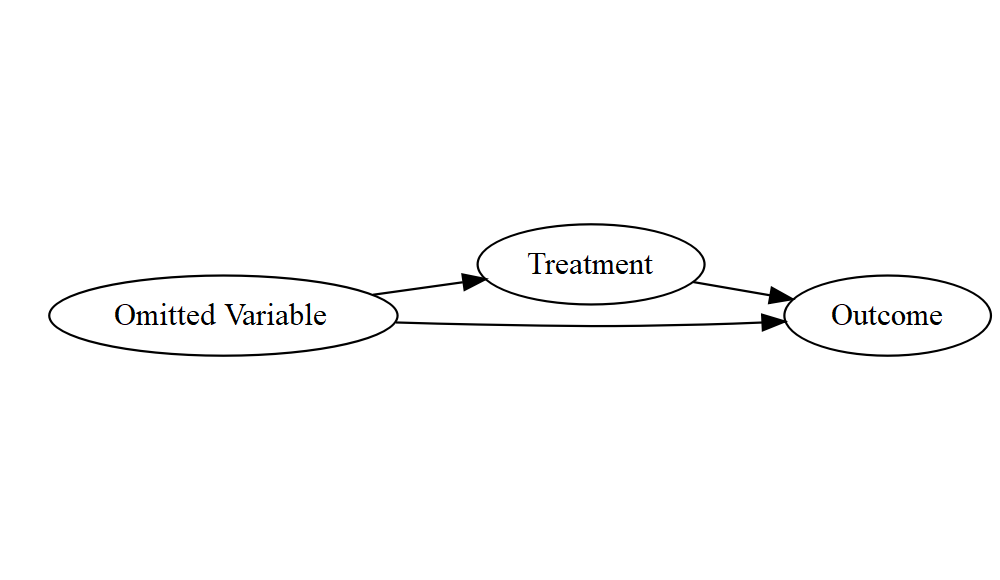
\includegraphics[width=\maxwidth]{figure/dag1-1} 

\end{knitrout}
\end{frame}

\begin{frame}
\frametitle{Instrumental Variables}
\begin{knitrout}
\definecolor{shadecolor}{rgb}{0.969, 0.969, 0.969}\color{fgcolor}
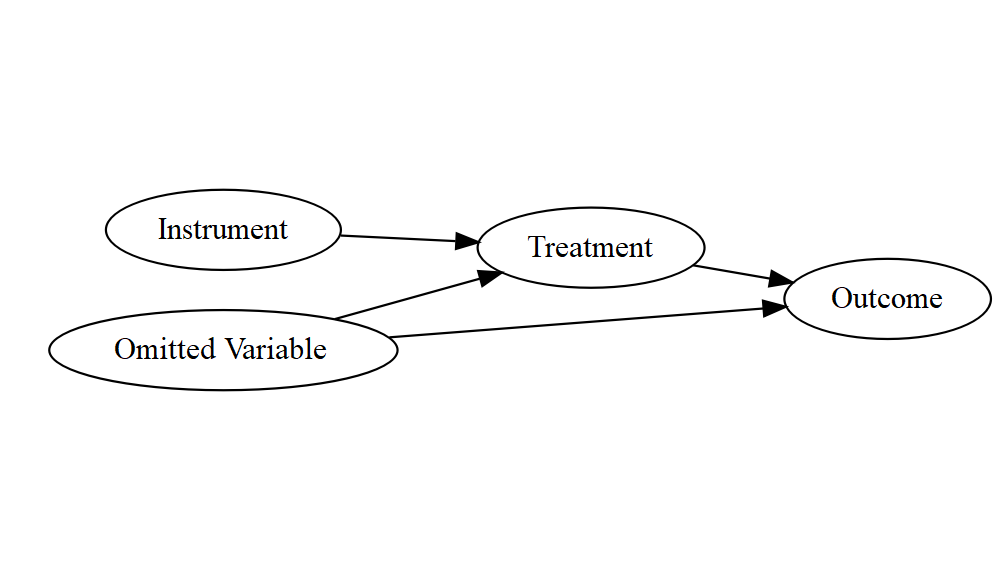
\includegraphics[width=\maxwidth]{figure/dag2-1} 

\end{knitrout}
\end{frame}

\begin{frame}
\frametitle{Instrumental Variables}
\begin{knitrout}
\definecolor{shadecolor}{rgb}{0.969, 0.969, 0.969}\color{fgcolor}
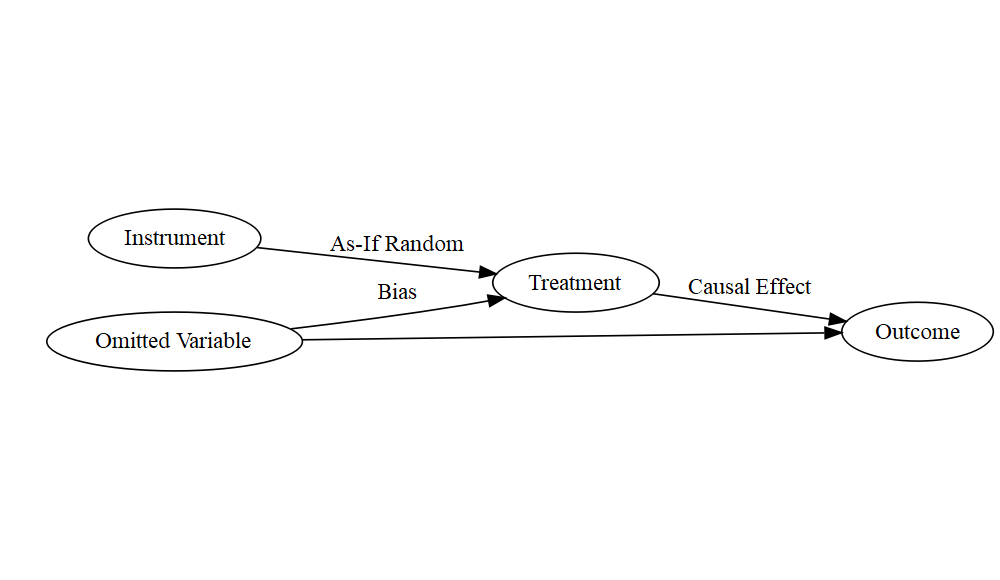
\includegraphics[width=\maxwidth]{figure/dag3-1} 

\end{knitrout}
\end{frame}

\begin{frame}
\frametitle{Instrumental Variables}
\begin{knitrout}
\definecolor{shadecolor}{rgb}{0.969, 0.969, 0.969}\color{fgcolor}
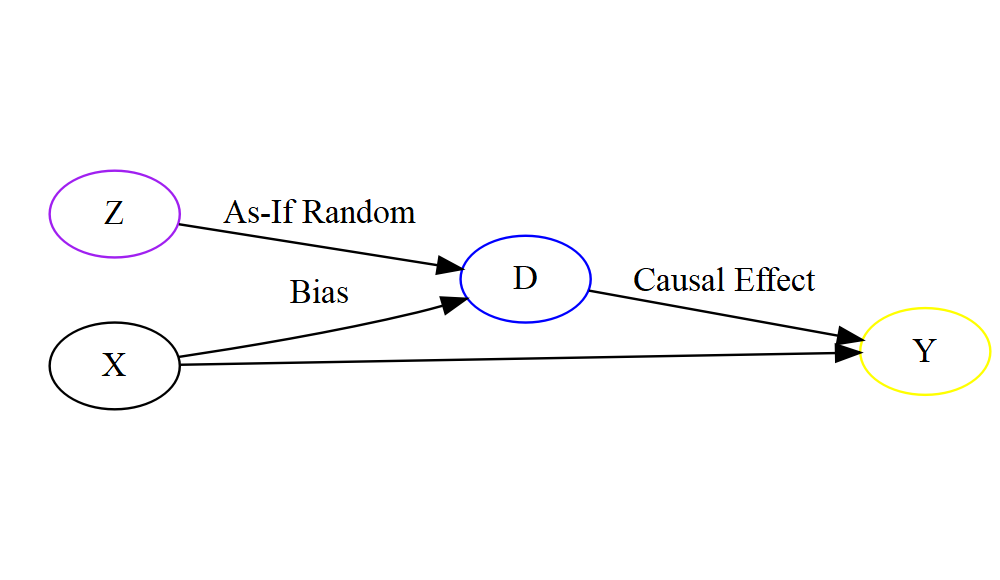
\includegraphics[width=\maxwidth]{figure/dag4-1} 

\end{knitrout}
\end{frame}


\begin{frame}
\frametitle{Instrumental Variables}
\begin{itemize}
\item Example Instruments:
\begin{itemize}
\item Rainfall for conflict 
\item Gender of first two children for effect of having a third child
\item Distance from the coast for exposure to slave trade
\end{itemize}
\end{itemize}
\end{frame}

\begin{frame}
\frametitle{Instrumental Variables Assumption}
\begin{multicols}{2}
\begin{itemize}
\item 1. \textbf{Strong 'First Stage':}
\pause
\item Instrument Predicts Treatment
\pause
\item We can assess this with a simple regression:
\pause
\item $D_i = \alpha + \beta Z_i + \epsilon_i$
\pause
\item The instrument should be a significant predictor of treatment
\pause
\item Rule-of-thumb: $F-statistic > 10$
\end{itemize}
\columnbreak
\begin{itemize}
\item 2. \textbf{Exclusion Restriction} 
\pause
\item The Instrument \textit{ONLY} affects the outcome through its effect on treatment, and not directly
\pause
\item Formally, $cov(Z_i, \epsilon_i \text{ in } Y_i \sim D_i)=0$
\pause
\item \textbf{We cannot test or prove this assumption!}
\pause
\item Theory and qualitative evidence needed
\end{itemize}
\end{multicols}
\end{frame}

\begin{frame}
\frametitle{Instrumental Variables Methodologies}
\begin{multicols}{2}
\begin{itemize}
\item 1. \textbf{2-Stage Least Squares (2SLS):}
\pause
\item Isolate the variation in treatment caused by the instrument: $D_i = \alpha + \beta_1 Z_i + \epsilon_i$
\pause
\item Save the predicted values from this regression: $\hat{D_i} = \hat{\alpha} + \hat{\beta_1} Z_i$
\pause
\item Estimate how the predicted values affect the outcome: $Y_i = \alpha + \beta_2 \hat{D_i}$
\pause
\item Interpret the coefficient on $\hat{D_i}$
\pause
\item But our Standard Errors won't be accurate
\end{itemize}
\columnbreak
\begin{itemize}
\item 2. \textbf{All-in-one Package} 
\pause
\item Use an all-in-one package, eg. \textit{ivreg} in the \textit{AER} package
\pause
\item Specify the formula: $Y_i \sim D_i | Z_i$
\pause
\item Interpret the coefficient on $D_i$
\end{itemize}
\end{multicols}
\end{frame}

\begin{frame}
\frametitle{Instrumental Variables}
\begin{itemize}
\item Types of IV Regressions:
\pause
\begin{enumerate}
\item \textbf{Biased Regression:} The regression ignoring omitted variable bias: $Y_i \sim D_i$
\pause
\item \textbf{First-Stage Regression:} Checking the instrument is valid: $D_i \sim Z_i$
\pause
\item \textbf{IV Regression:} All-in-one estimate of the effect of treatment on the outcome: $Y_i \sim D_i | Z_i$
\pause
\item \textbf{2-Stage Least Squares:} Two linear regressions: correct coefficient, wrong p-value: $D_i \sim Z_i, then Y_i \sim \hat{D_i}$
\pause
\item \textbf{Reduced-Form Regression:} Estimate of the Instrument on the Outcome, \textit{ignoring treatment}: $Y_i \sim Z_i$
\end{enumerate}
\end{itemize}
\end{frame}

\begin{frame}
\frametitle{Example}
\begin{itemize}
\item \textbf{Our research question:} How does conflict affect economic growth?
\pause
\item \textbf{Our instrument for treatment:} Rainfall (lack of)
\pause
\item \textbf{First Stage Regression:} $Conflict_i \sim \alpha + \beta_1 Rainfall_i + \epsilon_i$
\end{itemize}
\end{frame}

\begin{frame}
\frametitle{Example}
\begin{itemize}
\item \textbf{Our research question:} How does conflict affect economic growth?
\item \textbf{Our instrument for treatment:} Rainfall
\item \textbf{First-Stage Regression:} $Conflict_i = 0.12 - 0.1^{*} Rainfall_i + \epsilon_i$
\pause
\item \textbf{Fitted values from First-Stage Regression:} $\hat{Conflict_i} = 0.12 - 0.1^{*} 0.8 + \epsilon_i$
\end{itemize}
\end{frame}

\begin{frame}
\frametitle{Example}
\begin{itemize}
\item \textbf{Our research question:} How does conflict affect economic growth?
\item \textbf{Our instrument for treatment:} Rainfall
\item \textbf{First-Stage Regression:} $Conflict_i = 0.12 - 0.1^{*} Rainfall_i + \epsilon_i$
\item \textbf{Fitted values from First-Stage Regression:} $0.07 = 0.12 - 0.1^{*} 0.5$
\end{itemize}
\end{frame}

\begin{frame}
\frametitle{Example}
\begin{itemize}
\item \textbf{Our research question:} How does conflict affect economic growth?
\item \textbf{Our instrument for treatment:} Rainfall
\item \textbf{First-Stage Regression:} $Conflict_i = 0.12 - 0.1^{*} Rainfall_i + \epsilon_i$
\item \textbf{Fitted values from First-Stage Regression:} $\hat{Conflict_i} = 0.07, 0.02, 0.06, 0.12, 0.03...$
\pause
\item \textbf{Second-Stage Regression:} $Growth_i = \alpha + \beta_2 \hat{Conflict_i} + \epsilon_i$
\end{itemize}
\end{frame}

\begin{frame}
\frametitle{Example}
\begin{itemize}
\item \textbf{Our research question:} How does conflict affect economic growth?
\item \textbf{Our instrument for treatment:} Rainfall
\item \textbf{First-Stage Regression:} $Conflict_i = 0.02 + 0.1^{*} Rainfall_i + \epsilon_i$
\item \textbf{Fitted values from First-Stage Regression:} $\hat{Conflict_i} = 0.07, 0.02, 0.06, 0.12, 0.03...$
\item \textbf{Second-Stage Regression:} $Growth_i = 1.2 - 0.04^{*} \hat{Conflict_i} + \epsilon_i$
\end{itemize}
\end{frame}

\begin{frame}
\frametitle{LATE}
\begin{itemize}
\item IV Interpretation:
\pause
\begin{itemize}
\item Your coefficient is a causal estimate ONLY for units that were actually treated \textbf{because of the instrument}
\pause
\item They don't tell us about the causal effect for other units that \textit{never responded to the instrument}
\pause
\item Eg. For places where conflict started because of ethnic tensions or an accident
\end{itemize}
\end{itemize}
\pause
\begin{block}{Local Average Treatment Effect (LATE)}
The Average Treatment Effect among the subset of units who are treated because of the instrument: \\
$(D_i|Z_i=0) = 0$ and $(D_i|Z_i=1) = 1$
\end{block}
\begin{itemize}
\pause
\item Remember, these 'Local' units might be very rare and unusual so we can't generalize
\end{itemize}
\end{frame}

\section{Instrumenting for Institutions}

\begin{frame}
\frametitle{Instrumenting for Institutions}
\begin{itemize}
\item Acemoglu \& Robinson (2001)
\begin{itemize}
\item \textbf{Theory:} Non-electoral \textbf{institutions} (property rights, rule of law, checks and balances) cause economic growth
\pause
\end{itemize}
\item What is the inferential problem here?
\pause
\item Can we run a field experiment?
\pause
\item Can we find a natural experiment?
\end{itemize}
\end{frame}

\begin{frame}
\frametitle{Instrumenting for Institutions}
\begin{itemize}
\item They need an Instrumental Variable that:
\pause
\begin{enumerate}
\item \textbf{First Stage:} \pause Predicts Institutions
\pause
\item \textbf{Exclusion Restriction:} \pause Only affects growth through institutions
\end{enumerate}
\pause
\item They \textit{argue} that Settler (soldier) mortality rates are an appropriate instrument for institutions
\end{itemize}
\end{frame}


\begin{frame}
\frametitle{Instrumenting for Institutions}
\begin{itemize}
\item \textbf{Population:} \pause Ex-colonies
\pause
\item \textbf{Sample:} \pause Ex-colonies
\pause
\item \textbf{Treatment:} \pause 'Settler' Institutions in ex-colonies (measured by 'risk of expropriation' index 1985-95)
\pause
\item \textbf{Control:} \pause 'Extractive' institutions
\pause
\item \textbf{Outcome:} \pause Growth rates in 1995
\pause
\item \textbf{Treatment Assignment Mechniams:} \pause Messy! But high settler mortality rates led to extractive institutions
\pause
\item \textbf{Instrument:} \pause Settler (soldier) mortality rates
\end{itemize}
\end{frame}

\begin{frame}
\frametitle{Instrumenting for Institutions}
\begin{itemize}
\item \textbf{First Stage:} \pause Settler mortality rates predict institutions
\pause
\item Supporting Evidence:
\pause
\item ``Mortality rates faced by the settlers more than 100 years ago explains over 25 percent of the variation in current institutions.''
\end{itemize}
\end{frame}

\begin{frame}
\frametitle{Instrumenting for Institutions}
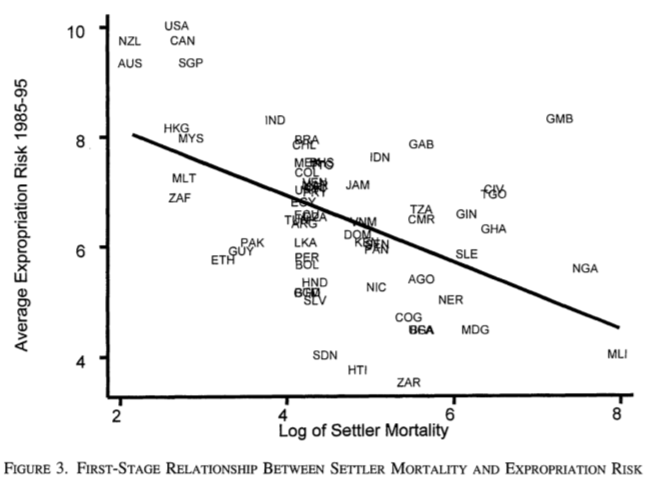
\includegraphics[scale=0.38]{AJR_first_stage.png}
\end{frame}

\begin{frame}
\frametitle{Instrumenting for Institutions}
\begin{itemize}
\item \textbf{Exclusion Restriction:} \pause Settler mortality rates ONLY affect growth through institutions
\pause
\item Supporting Evidence:
\begin{itemize}
\item Mortality rates for locals are low and don't affect human capital/growth directly, due to local immunity
\pause
\item Control for other possible correlated variables - geography, climate, etc.
\end{itemize}
\end{itemize}
\end{frame}

\begin{frame}
\frametitle{Instrumenting for Institutions}
\begin{itemize}
\item Methodology:
\begin{itemize}
\item ${\color{blue}Institutions_i} = \alpha + \beta_0 Settler\_Mortality_i + \epsilon_i$
\item $Growth_i = \alpha + \beta_1 {\color{blue}\hat{Institutions_i}} + \epsilon_i$
\end{itemize}
\end{itemize}
\end{frame}

\begin{frame}
\frametitle{Instrumenting for Institutions}
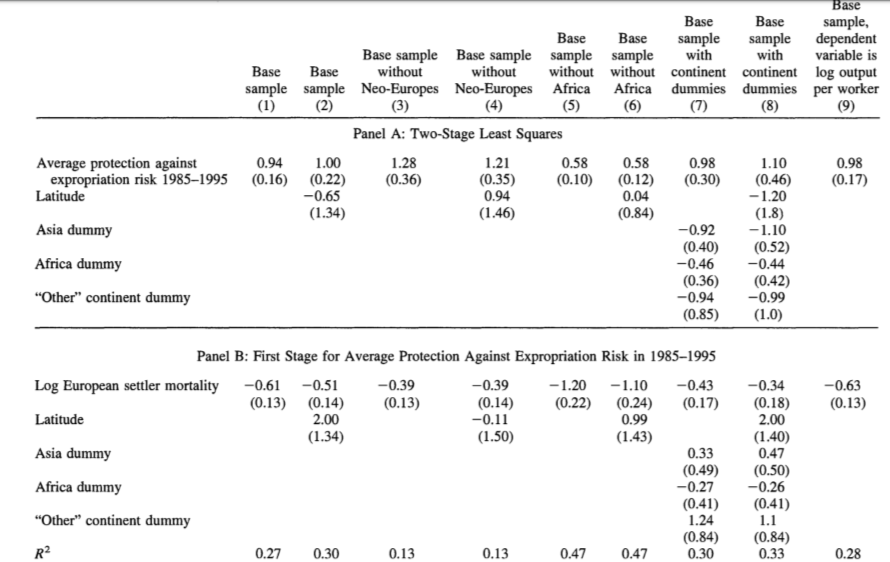
\includegraphics[scale=0.36]{AJR_results.png}
\end{frame}

\begin{frame}
\frametitle{Instrumenting for Institutions}
\begin{itemize}
\item \textbf{Results:} Improving Nigeria's institutions to Chile's level would raise GDP 7-fold
\end{itemize}
\end{frame}

\section{Non-Compliance in Experiments}

\begin{frame}
\frametitle{Non-Compliance in Experiments}
\begin{itemize}
\item Sometimes field experiments don't work perfectly
\pause
\begin{itemize}
\item Eg. We offer free health insurance to families at random, but some decline
\pause
\item What is the Treatment Assignment Mechanism?
\pause
\item Those that decline treatment are \textit{different} to those that accept (eg. richer)
\pause
\end{itemize}
\item We cannot just compare units that actually received treatment to those that did not
\pause
\item Those groups are no longer 'balanced'
\pause
\item Omitted variable bias has returned!
\end{itemize}
\end{frame}

\begin{frame}
\frametitle{Non-Compliance in Experiments}
\begin{table}[htbp]
  \centering
    \begin{tabular}{l|r|r}
    Income & \multicolumn{1}{l}{Treatment Assignment} & \multicolumn{1}{l}{Treatment Status} \\
    \hline
    Rich  & 1     & 0 \\
    Poor  & 0     & 0 \\
    Poor  & 0     & 0 \\
    Poor  & 1     & 1 \\
    Rich  & 1     & 0 \\
    Poor  & 0     & 0 \\
    Poor  & 1     & 1 \\
    Rich  & 0     & 0 \\
    Poor  & 0     & 0 \\
    \end{tabular}%
  \label{tab:addlabel}%
\end{table}%
\end{frame}

\begin{frame}
\frametitle{Non-Compliance in Experiments}
\begin{itemize}
\item We can divide our units into four types depending on how they accept or reject treatment assignment:
\end{itemize}
\begin{table}[htbp]
  \centering
    \begin{tabular}{|p{3cm}|p{3cm}|p{3cm}|}
    \hline
    \multicolumn{1}{|p{3cm}|}{\textbf{If Assigned to Control}} & \multicolumn{1}{p{3cm}|}{\textbf{If Assgined to Treatment}} & \textbf{Unit Type} \bigstrut\\
    \hline
    0     & 1     & Complier \bigstrut\\
    \hline
    0     & 0     & Never-taker \bigstrut\\
    \hline
    1     & 1     & Always-taker \bigstrut\\
    \hline
    1     & 0     & Defier \bigstrut\\
    \hline
    \end{tabular}%
  \label{tab:addlabel}%
\end{table}%
\end{frame}

\begin{frame}
\frametitle{Non-Compliance in Experiments}
\begin{table}[htbp]
  \centering
    \begin{tabular}{c|c|c}
    \multicolumn{1}{l}{$D_i(Z_i=0)$} & \multicolumn{1}{l}{$D_i(Z_i=1)$} & \multicolumn{1}{l}{} \\
    \hline
    \multicolumn{1}{l}{If Assigned to Control} & \multicolumn{1}{l}{If Assigned to Treatment} & \multicolumn{1}{l}{Type?} \\
    \hline
    0     & 1     &  \\
    0     & 0     &  \\
    0     & 1     &  \\
    1     & 0     &  \\
    1     & 1     &  \\
    0     & 0     &  \\
    0     & 1     &  \\
    1     & 0     &  \\
    \end{tabular}%
  \label{tab:addlabel}%
\end{table}%

\end{frame}

\begin{frame}
\frametitle{Non-Compliance in Experiments}
\begin{itemize}
\item Simple difference-in-means estimates are biased
\pause
\item But we can still use the randomized component of \textbf{treatment assignment as an instrumental variable}
\pause
\end{itemize}
\begin{block}{Local Average Treatment Effect (LATE)}
The Average Treatment Effect among Compliers
\end{block}
\begin{itemize}
\item LATE just means we don't learn anything about Never-takers and Always-takers from our Instrumental Variable
\pause
\begin{itemize}
\item Because the instrument doesn't do anything to affect treatment for these units
\end{itemize}
\pause
\item Never-takers and Always-takers are balanced across treatment assignment and do not affect the difference-in-means
\pause
\item We also need to \textbf{assume} Defiers don't exist
\end{itemize}
\end{frame}

\begin{frame}
\frametitle{Non-Compliance in Experiments}
\begin{itemize}
\item Two methodologies for Experiments with Non-Compliance
\end{itemize}
\begin{multicols}{2}
\begin{itemize}
\item \textbf{1. Intention-to-Treat Analysis}
\pause
\item The Effect of Treatment \textbf{Assignment} (the Instrument) on the Outcome
\pause
\item $Y_i ~ \alpha + \beta Z_i + \epsilon_i$
\pause
\item A BIASED estimate (<LATE estimate)
\pause
\item For the FULL sample
\end{itemize}
\columnbreak
\begin{itemize}
\item \textbf{2. LATE Instrumental Variables Analysis}
\pause
\item The Effect of Treatment on the Outcome
\pause
\item $Y_i ~ \alpha + \beta D_i|Z_i + \epsilon_i$
\pause
\item An UNBIASED estimate
\pause
\item Only for COMPLIERS
\end{itemize}
\end{multicols}
\end{frame}

\begin{frame}
\frametitle{Non-Compliance in Experiments}
\begin{itemize}
\item The \textbf{'Strong First-Stage'} assumption here requires that treatment assignment affects treatment for at least some people
\pause
\item The \textbf{'Exclusion Restriction'} assumption requires that outcomes depend on treatment and not treatment assignment
\begin{itemize}
\item So being labelled 'treatment' doesn't affect your attitude to redistribution
\end{itemize}
\end{itemize}
\end{frame}


\end{document}
